The user selects the artist's biography (for completeness) and birth (for validation). \karma automatically constructs SPARQL queries to retrieve the data, integrates it into the worksheet, and augments the \rtworml mapping accordingly (Figure~\ref{fig:augment-screenshot}). 
To support the integrated SPARQL queries, we generated owl:sameAs links between the artists in the CSV file and the Smithsonian dataset using LIMES \cite{ngomo2011limes} (we plan to integrate LIMES with \karma to enable users to perform all integration steps within \karma). 
\begin{figure*}[htb]
\centering
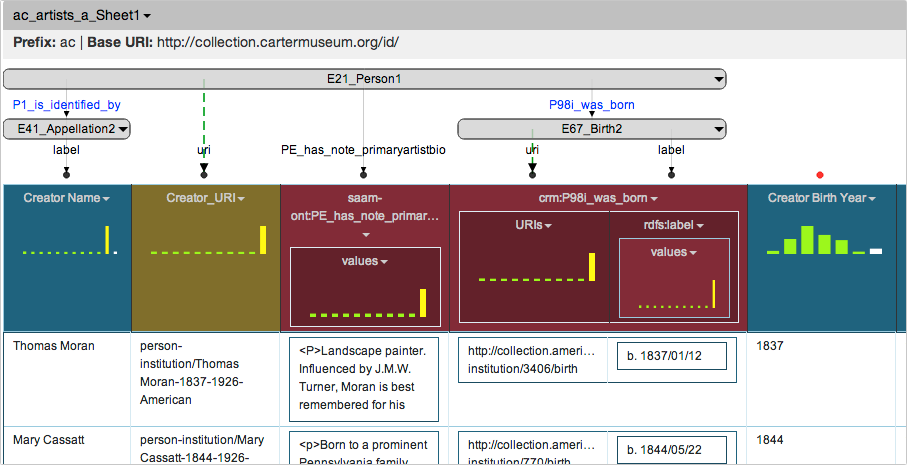
\includegraphics[width=4.9in]{images/6-augment.png}
\vspace{-5mm}
\caption{A Karma user has integrated biographical data from the Smithsonian as new columns in their dataset. The columns contain artists' biographies and birth dates.}
\vspace{-15pt}
\label{fig:augment-screenshot}
\end{figure*}